\section{Results}

\subsection{Model calibration}

\begin{figure}
  \centering
  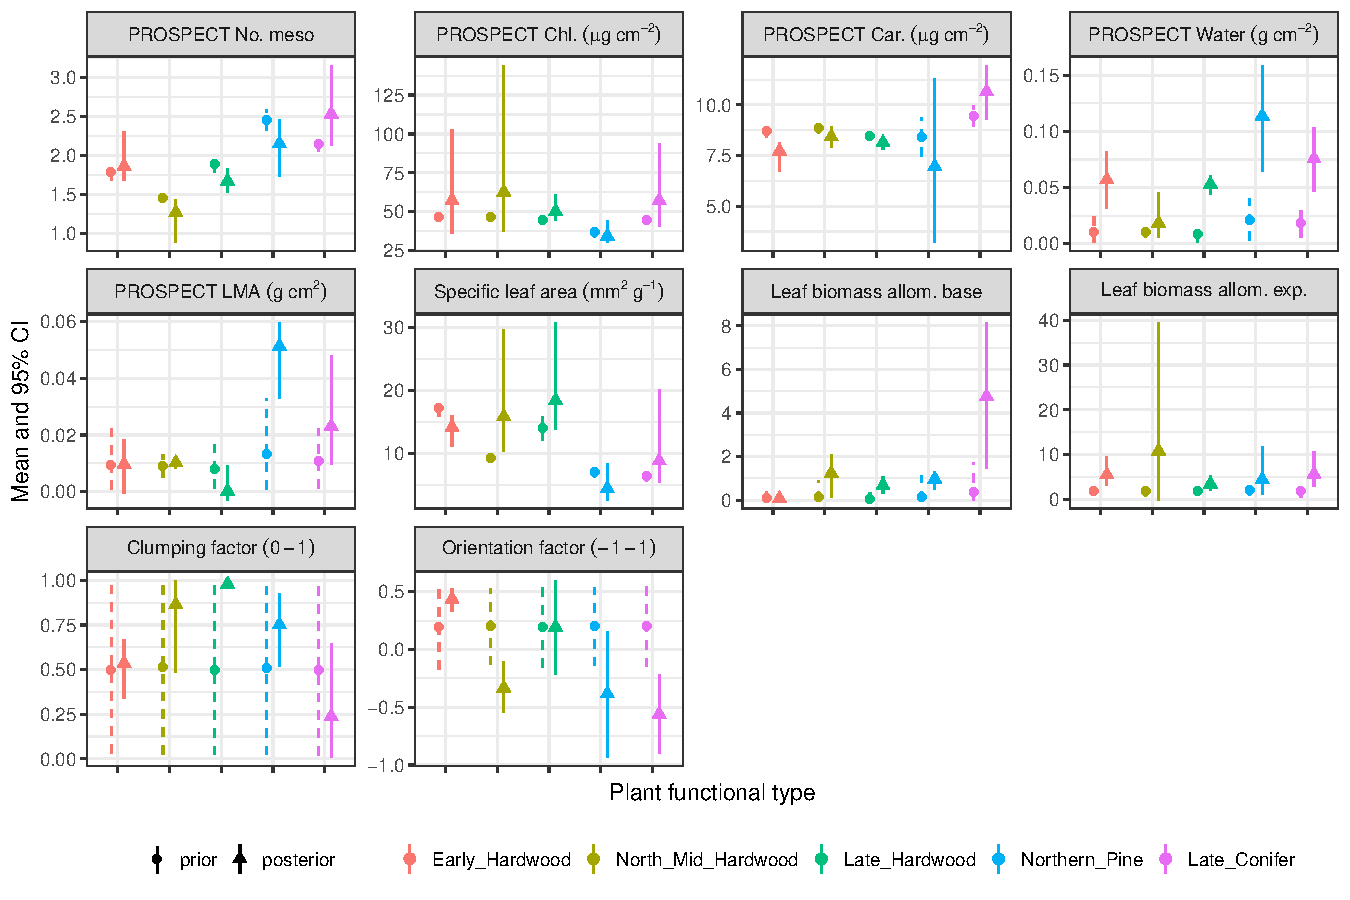
\includegraphics[width=\textwidth]{figures/pda_summary.pdf}
  \caption{\
    Summary statistics for model calibration parameter prior and posterior distributions.
  }\label{fig:pda_posteriors}
\end{figure}

Marginal posterior distributions on parameters with highly informative priors (PROSPECT parameters, SLA, and leaf allometries) generally had higher uncertainty than prior distributions.
However, the orientation factor and especially the clumping factor were somewhat more constrained relative to their priors.
Analyis of joint posterior distributions reveals very tight covariance between many parameters and across PFTs, which explains the much tighter spectral confidence intervals relative to the prior (see Supplementary Information).

\begin{figure}
  \centering
  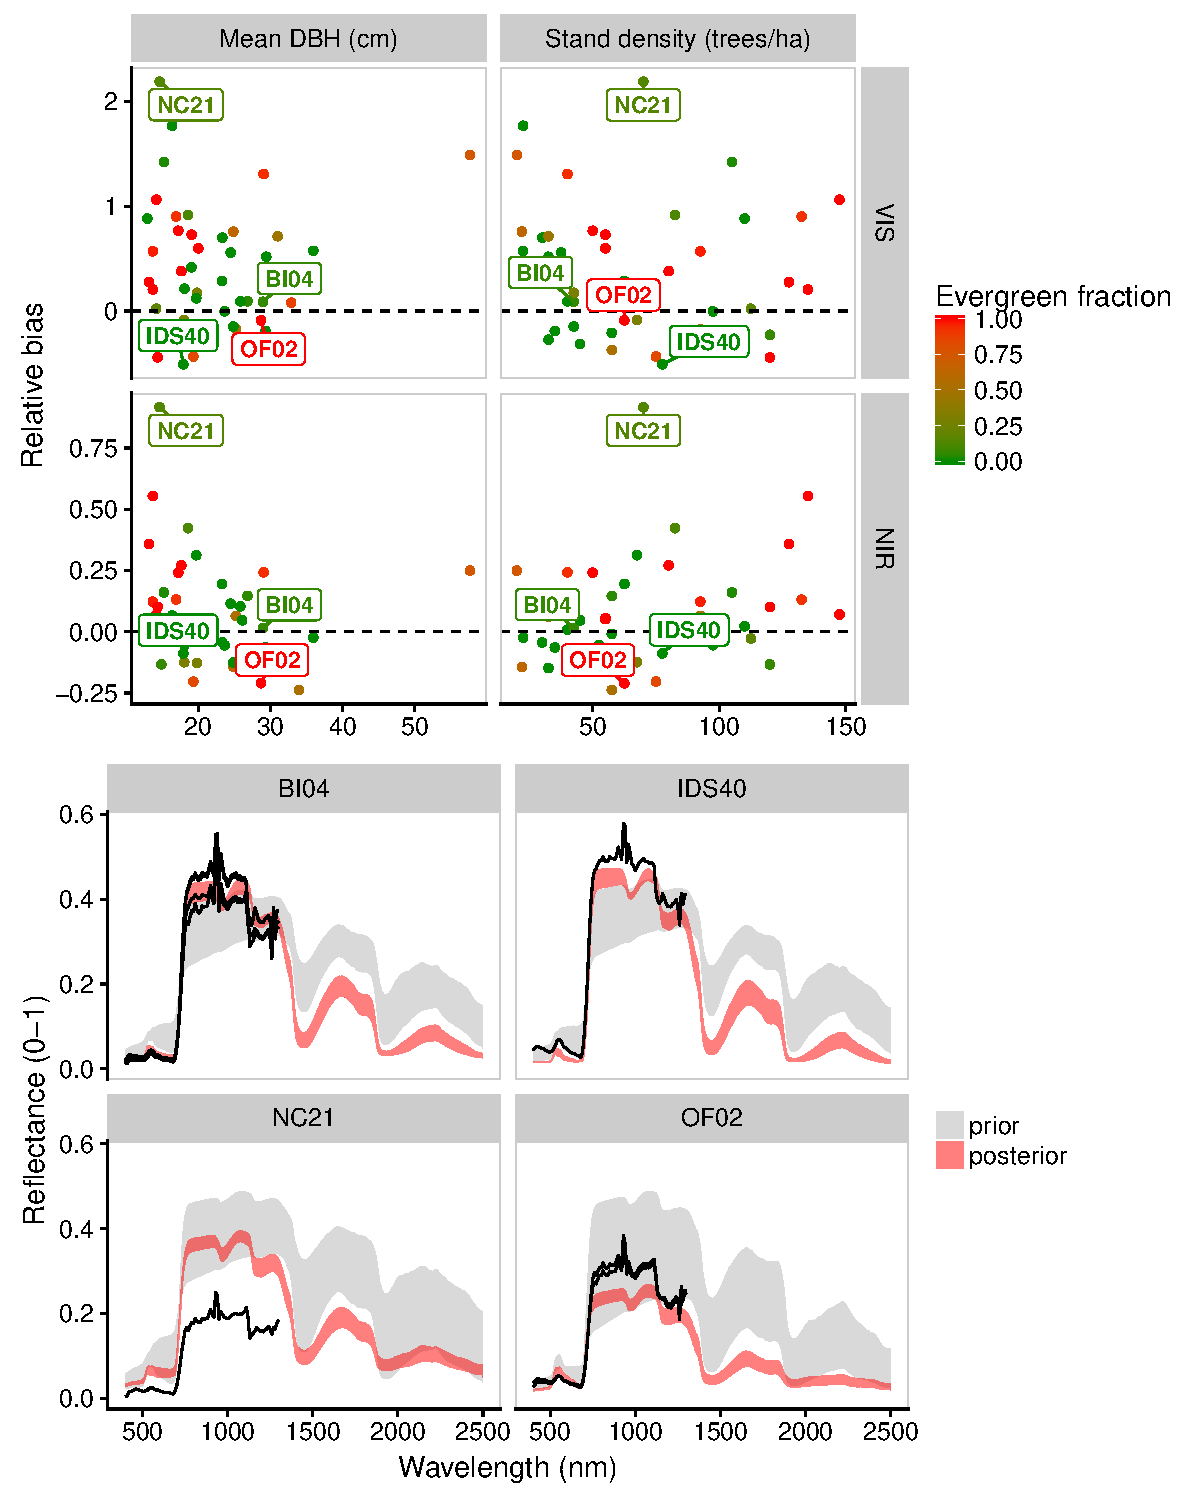
\includegraphics[width=\textwidth]{4_edr/figures/spec_validation.pdf}
  \caption{\
    (\textit{Top}) Relative bias of the posterior mean spectra at each site, aggregated across the visible (VIS, 400--750 nm) and near-infrared (NIR, 750--1300 nm) spectral range
    as a function of site mean diameter at breast height and stand density.
    (\textit{Bottom}) Prior and posterior predictive intervals and AVIRIS observations for four sites representative of different kinds of error.
  }\label{fig:bias}
\end{figure}

In general, after calibration across a large number of structurally and functionally diverse sites, EDR was able to reproduce observed AVIRIS canopy reflectance reasonably well.
However, performance was strongly site specific.
At many sites, but most prominently those composed of small trees (DBH < 20, e.g.\ site NC21), EDR frequently overestimated canopy reflectance.
That being said, least-squares linear regressions of relative spectral bias as a function of site mean DBH or stand density were not statistically significant ($p > 0.1$).
EDR was generally more likely to overestimate canopy reflectance for conifer trees than broadleaved trees.

\begin{figure}
  \centering
  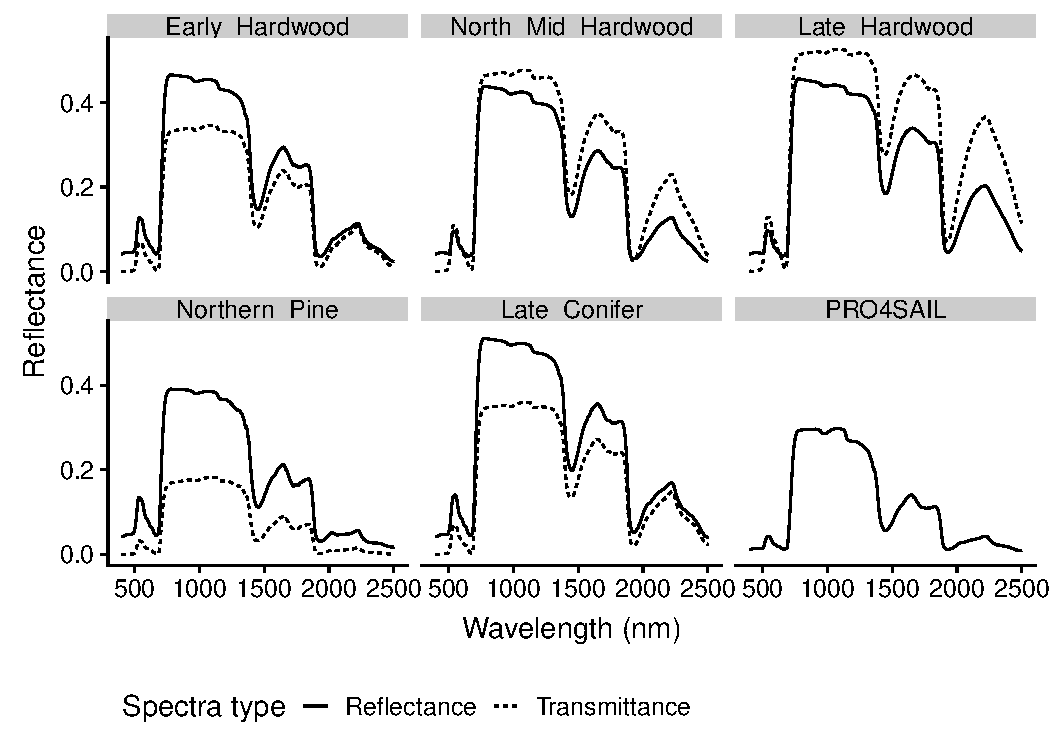
\includegraphics[width=\textwidth]{4_edr/figures/explore_spectra/pft_prospect_sim.pdf}
  \caption{%
    First five panels are PROSPECT simulations of leaf reflectance and transmittance for the plant functional types used in this analysis, based on parameters at their posterior means.
    The final panel is a simulation using the PRO4SAIL~\cite{verhoef_1984_sail} canopy radiative transfer model, parameterized with default structural parameters and leaf parameters averaged across the posterior means of the five plant functional types.
    % TODO: Add SAIL simulation
  }
\end{figure}

\begin{figure}
  \centering
  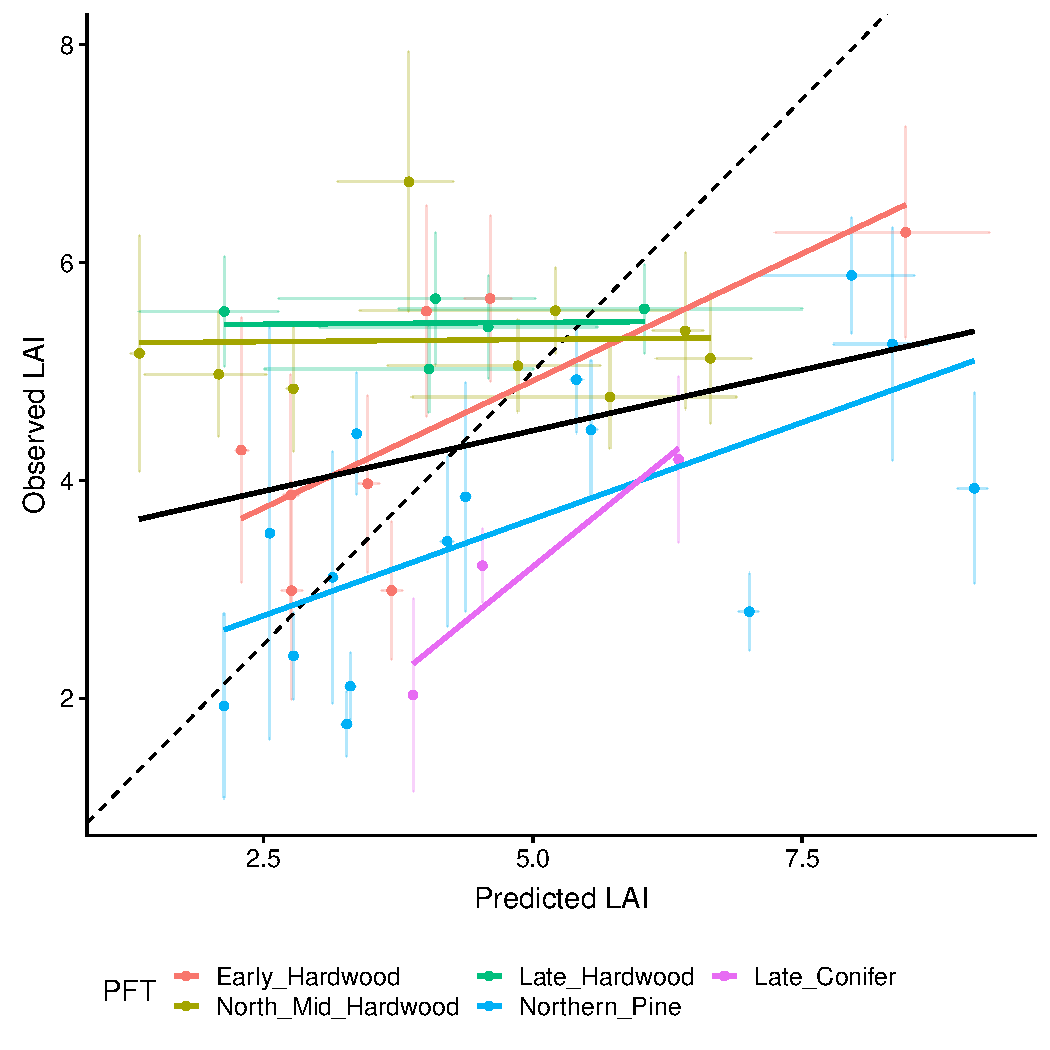
\includegraphics[width=\textwidth]{4_edr/figures/explore_spectra/lai_scatter.pdf}
  \caption{\
    Predictions of leaf area index by EDR, compared to observed values.
    Colors indicate the plant functional type of the tallest cohort at each site.
    % TODO: Add by-PFT regression line
  }\label{fig:lai_validation}
\end{figure}

\begin{figure}
  \centering
  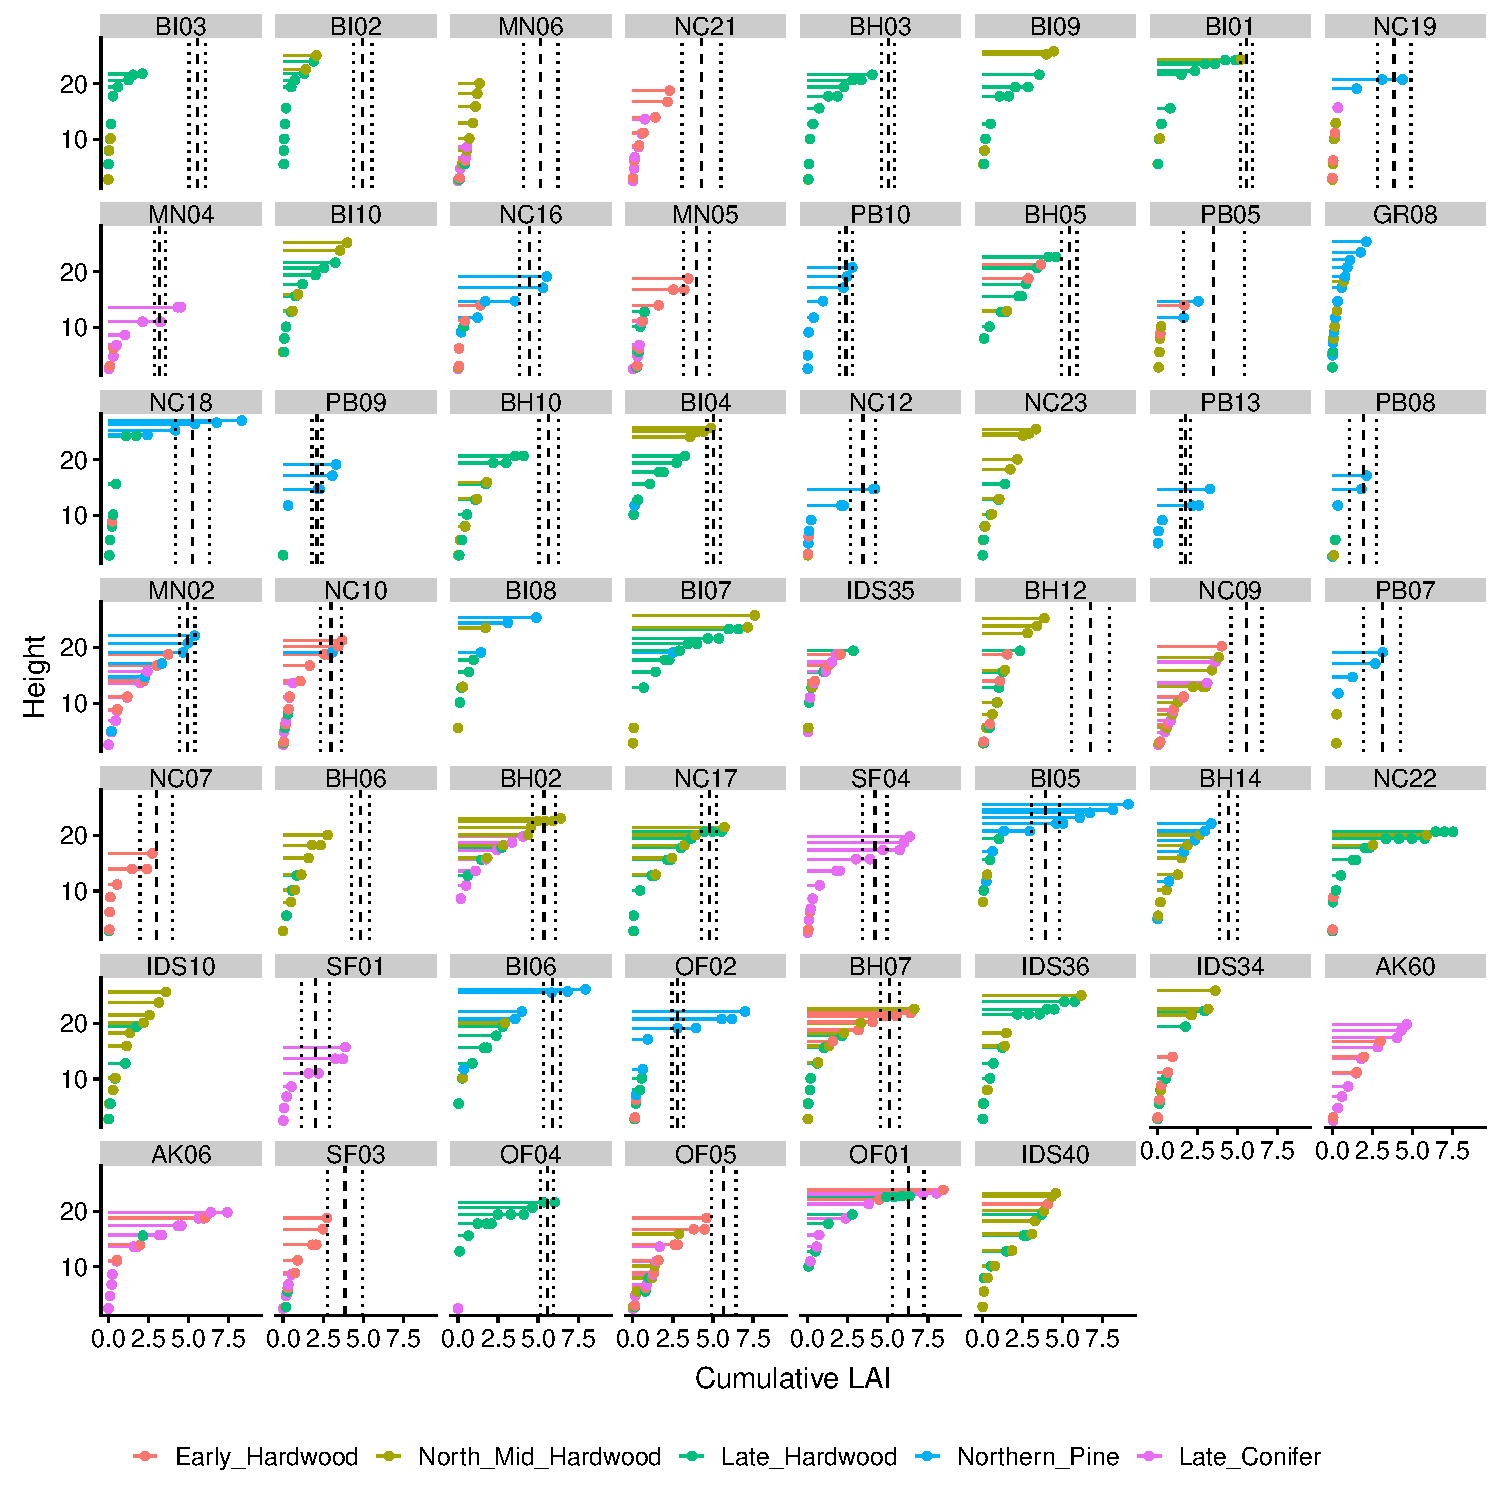
\includegraphics[width=\textwidth]{4_edr/figures/explore_spectra/ed_cumlai_plot.pdf}
  \caption{%
    Vertical profile of cumulative leaf area index and composition at each site in this analysis.
    Vertical black lines indicate the mean $\pm$ 1 standard deviation of the observed leaf area index.
  }
\end{figure}

EDR predictions of LAI also agreed reasonably well with observations for most sites.
EDR tended to overestimate LAI for conifer-dominated stands and slightly underestimate it for deciduous stands.

%\begin{figure}
  %\centering
  %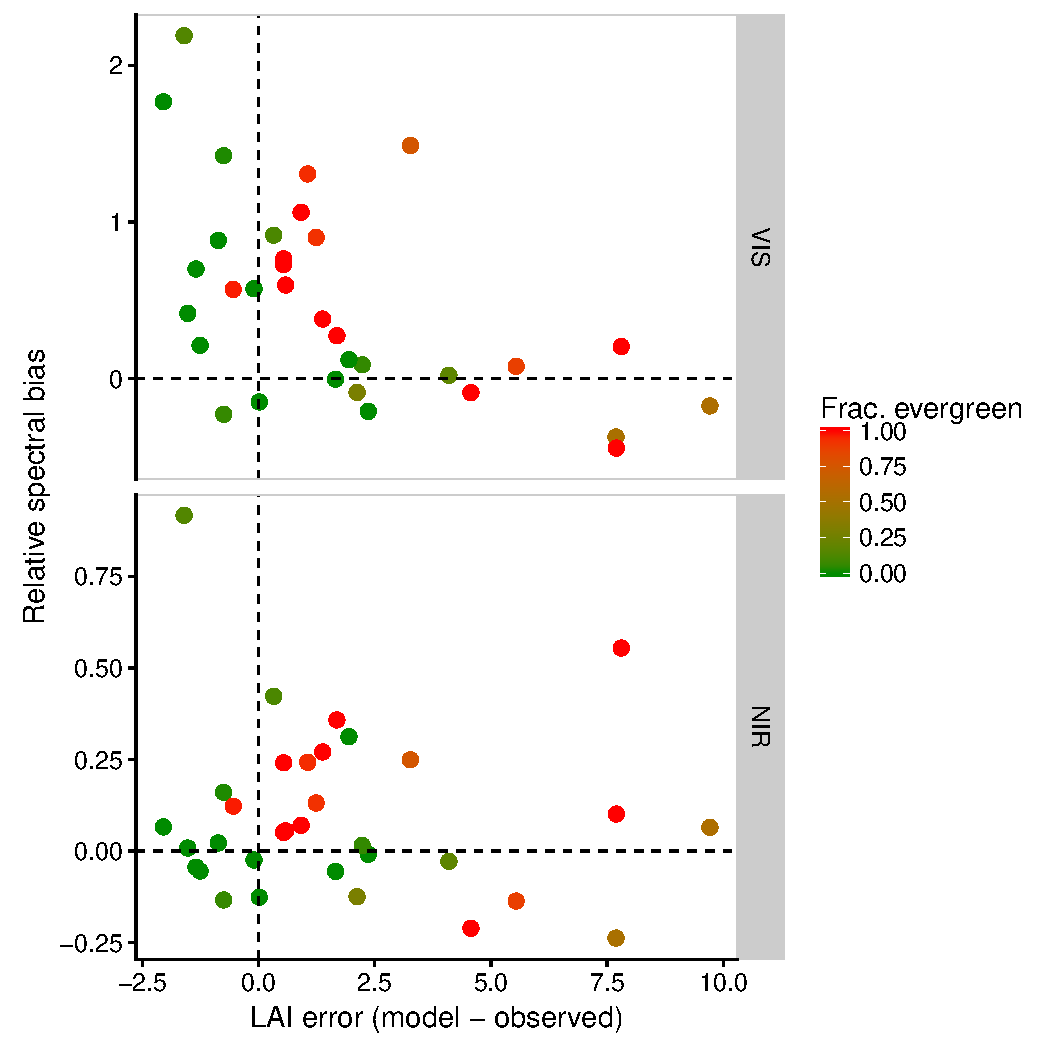
\includegraphics[width=\textwidth]{figures/spec_lai.pdf}
  %\caption{\
    %Relationship between errors in EDR predictions of leaf area index and spectra.
  %}\label{fig:spec_lai}
%\end{figure}

%There was a significant negative relationship between EDR LAI errors and spectral errors in the visible range;
%in other words, EDR tended to overestimate either LAI or canopy reflectance.

\subsection{Forward simulation}

\begin{figure}
  \centering
  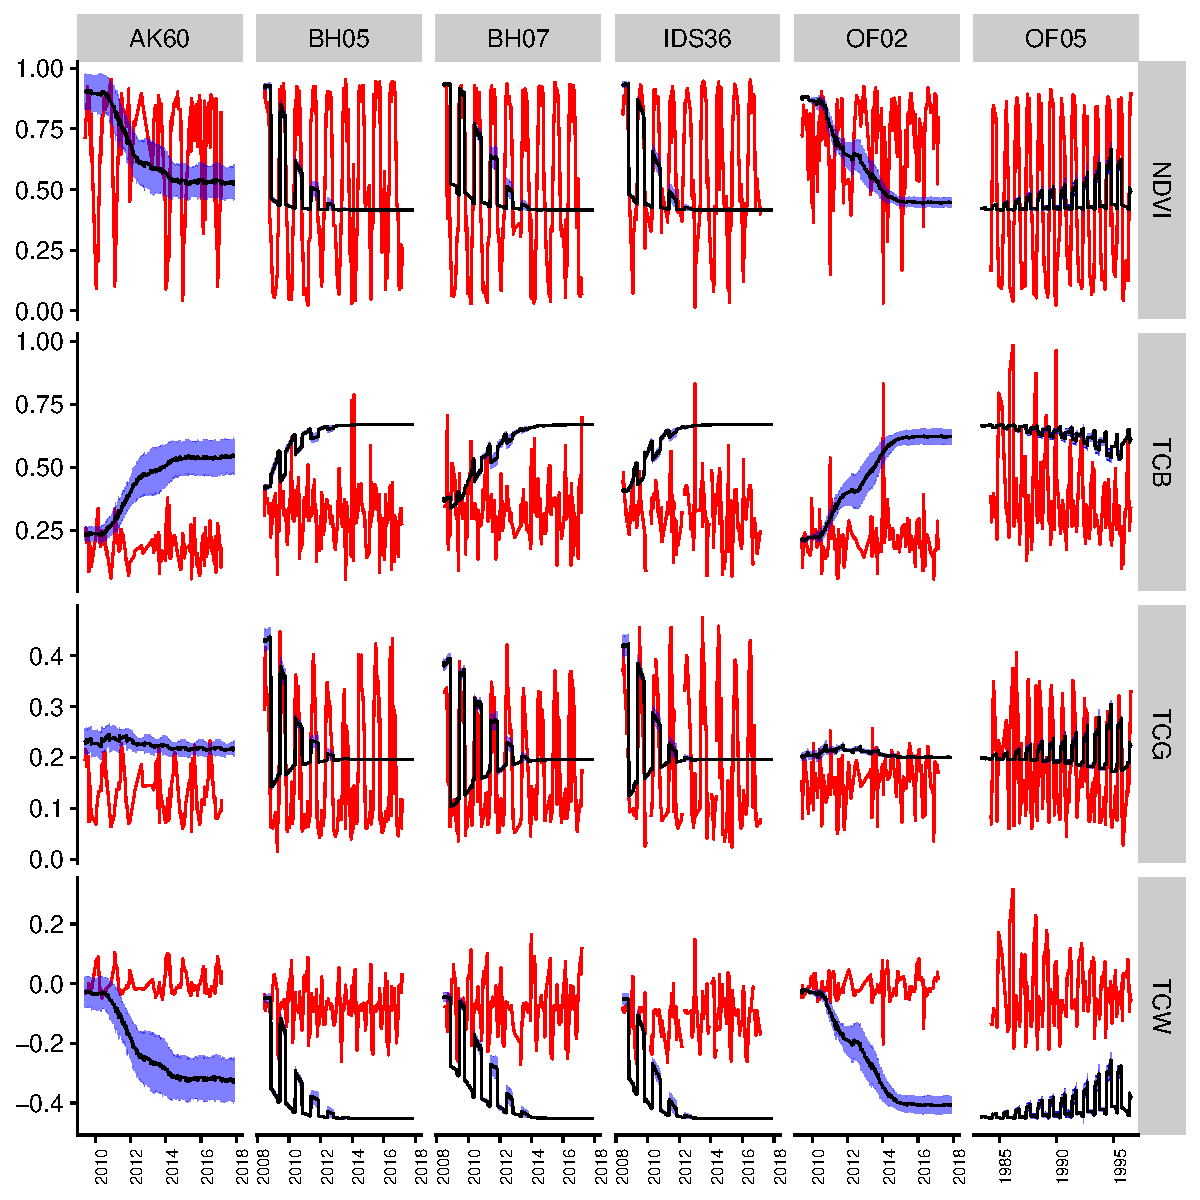
\includegraphics[width=\textwidth]{figures/landsat_ts.pdf}
  \caption{\
    Comparison of EDR-simulated (black, blue ribbon) and observed (red) time series of Landsat NDVI and tasseled cap brightness (TCB), greenness (TCG), and wetness (W) for each site.
  }
\end{figure}

(Currently working on this text\ldots).
